\documentclass[a4paper, 14pt]{extarticle}
\setlength{\parindent}{0.75cm}
\usepackage[utf8]{inputenc}
\usepackage[T2A]{fontenc}
\usepackage[warn]{mathtext}
\usepackage{amssymb}
\usepackage{amsmath}
\usepackage[russian]{babel}
\usepackage{scrextend}
\usepackage{multirow}
\usepackage{hhline}
\usepackage{float}
\usepackage{multicol}
\usepackage{graphicx}
\usepackage{placeins}
\usepackage{makecell}
\usepackage{setspace}
\usepackage{ragged2e}
\usepackage{titlesec}
\usepackage{listings}
\usepackage{svg}
\usepackage{xcolor}
\usepackage{tocloft}
\usepackage[left=2cm,right=2cm, top=2cm,bottom=2cm,bindingoffset=0cm]{geometry}
\usepackage{hyperref}
\hypersetup{
    colorlinks=true,
    linkcolor=blue,
    urlcolor=blue,
    citecolor=blue
}

\lstset{
  language=matlab,
  basicstyle=\ttfamily\small,
  keywordstyle=\color{blue},
  stringstyle=\color{red},
  commentstyle=\color{green},
  identifierstyle=\color{black},
  showstringspaces=false,
  showspaces=false,
  showtabs=false,
  numbers=left,
  numbersep=5pt,
  breaklines=true,
  breakatwhitespace=true,
  frame=single,
  rulecolor=\color{gray},
  backgroundcolor=\color{gray!5},
  captionpos=b,
  tabsize=2
}

\newcommand{\myappendixsection}[1]{%
  \section*{\large #1}
}

			
\usepackage[T2A]{fontenc}			
\usepackage[russian]{babel}			
\usepackage[utf8x]{inputenc}			
\usepackage[scaled=0.95]{PTSans}			
\usepackage{graphicx}			
%\usepackage[usenames,dvipsnames]{xcolor}			
\usepackage{algorithm}			
\usepackage{algorithmic}			
\usepackage{latexsym,amssymb,amsthm}			
%предметный указатель

\usepackage{multicol}

\newenvironment{theindex}{}{}

\usepackage[xindy]{imakeidx}

\renewenvironment{theindex}{%
	
	
	
	\vspace*{-25pt}\begin{center}\color{blue}\Large Предметный указатель\end{center}%
	
	
	
	\def\item{\par\hangindent 0pt\parindent0pt}%
	
	\def\subitem{\par\hangindent10pt\parindent10pt}%
	
	\def\subsubitem{\par\hangindent20pt\parindent20pt}%
	
	\def\indexspace{}%
	
	\begin{multicols}{2}
		
	}{\end{multicols} }



\makeindex[options=-L russian -C utf8]

\AtBeginDocument{%
	
	\let\originalindex\index
	
	\renewcommand{\index}[1]{\originalindex{\detokenize{#1}}}%
	
}

%конец предметного указателя			
\usepackage{ragged2e}			
\justifying			
\renewcommand{\raggedright}{\leftskip=0pt \rightskip=0pt plus 0cm}			
\hyphenpenalty=5 			
\exhyphenpenalty=10000			
\doublehyphendemerits=2			
\finalhyphendemerits=500			
\uchyph=0			
\renewcommand{\algorithmicrequire}{\textbf{Вход:}}			
\renewcommand{\algorithmicensure}{\textbf{Выход:}}			
\renewcommand{\algorithmiccomment}{{\color{gray} //}}			
%Здесь располагаются все макросы для всякой математики и алгоритмов -			
%\let\em\it			
\def\em#1{{\it\color{blue}#1}}
\def\NB#1{{\bf\color{brown}#1}}
\def\RS{{\color{red}\bf*}}	
\def\BS{{\color{blue}\bf*}}		
%\def\eqed{\tag{\qed}}			
\def\Boxed#1{#1}			
\def\odmkey#1#2{{\it\color{red} #1}\index{#2}}			
\let\emptyset\varnothing			
\def\Set#1#2{\left\{ #1 \mid #2 \right\}}			
\let\Equiv\Longleftrightarrow			
\def\Assign{\operatorname{:=}}			
\def\Pointer{\operatorname{\uparrow\!}}			
\def\Is{\operatorname{\colon}}
\def\plusplus{\operatorname{+\!+}}			
\def\Def{\stackrel{\text{Def}}{=}}			
\def\SubsetNE{\varsubsetneq}%\stackrel{\ne}{\subset}}			
\def\SubsetOne{\stackrel{+1}{\subset}}			
\def\dDef{\operatorname{::=}}			
\def\A#1#2{\forall\,#1\ \left(#2\right)}			
%\def\A#1#2{\forall\,#1\ \linebreak[2]\left(#2\right)}			
\def\dA#1#2{\forall\,#1\cdots #2}			
\def\Alg#1#2{\left\langle #1;#2\right\rangle}			
\def\Bl#1{\mathbf{#1}}			
\def\hy#1{\left( #1 \right)}			
\def\DIVC#1#2{\left\langle #1 , #2\right\rangle}
\def\divC#1#2{\left\langle #1 , #2\right\rangle}			
\def\DIVI#1#2{#1\in #2}			
\def\E#1#2{\exists\,#1\ \left(#2\right)}			
%\def\E#1#2{\exists\,#1\ \linebreak[2]\left(#2\right)}			
\def\To#1{\stackrel{#1}{\longrightarrow}}			
\def\ToC#1{\stackrel{#1}{,}}			
\def\ToS#1{\stackrel{#1}{\sim}}			
\def\ToE#1{\stackrel{#1}{=}}			
\def\Tuple#1#2#3{{#1}_{#2},\dots,{#1}_{#3}}			
\def\dTuple#1#2#3{{#1}_{#2}\dots{#1}_{#3}}			
\let\Impl\Longrightarrow			
\let\Impll\Longleftarrow			
\def\And{\operatorname{\,\&\,}}			
\def\Or{\,\vee\,}			
\def\Wedge{\,\wedge\,}			
\def\BigOr{\bigvee}			
\def\BigAnd{\bigwedge}			
\def\nat{\operatorname{\rm nat}}			
\def\sgn{\operatorname{\rm sgn}}			
\def\func{\operatorname{\rm func}}			
\def\ker{\operatorname{\rm ker}}			
\def\Im{\operatorname{\rm Im}}			
\def\Dom{\operatorname{\rm Dom}}			
\def\Ob{\operatorname{\rm Ob}}			
\def\Mor{\operatorname{\rm Mor}}			
\def\SetCat{\operatorname{\rm Set}}			
\def\OrSet{\operatorname{\rm OrSet}}			
\def\Aut{\operatorname{\rm Aut}}			
\def\End{\operatorname{\rm End}}			
\def\Gr{\operatorname{\rm Gr}}			
\def\Suc{\operatorname{\rm Suc}}			
\def\card{\operatorname{\rm card}}			
\def\pr{\operatorname{\rm pr}}			
\def\MOD{\operatorname{\rm\bf mod}}			
\def\DIV{\operatorname{\rm\bf div}}			
\def\Lrf#1{\lfloor #1 \rfloor}			
\def\lrle#1{\langle #1 \rangle}			
\def\llrle#1{\langle {\text{#1}} \rangle}			
\def\Map#1#2#3{{#1}\colon{#2}\nolinebreak\to\nolinebreak{#3}}			
\def\MapI#1#2#3{{#1}\colon{#2}\in{#3}}			
\def\Rule#1#2#3{\frac{#1}{#2}\,#3}			
\def\Seq#1#2#3{#1 \vdash_{#3} #2}			
\def\Prog#1#2#3{\{#1\}\,#2\,\{#3\}}			
\def\Not{\neg}			
\def\demo{\noindent $\triangleright$ \vskip 3 em \par\hfill$\triangleleft$}			
\DeclareMathOperator{\Eq}{Eq}			
\DeclareMathOperator{\Unify}{Unify}			
\DeclareMathOperator{\Antilex}{Antilex}			
\DeclareMathOperator{\Reverse}{Reverse}			
\DeclareMathOperator{\Fano}{Fano}			
\DeclareMathOperator{\Med}{Med}			
\DeclareMathOperator{\Huffman}{Huffman}			
\DeclareMathOperator{\Up}{Up}			
\DeclareMathOperator{\Down}{Down}			
\DeclareMathOperator{\KCC}{KCC}			
\DeclareMathOperator{\NewNode}{NewNode}			
\DeclareMathOperator{\Find}{Find}			
\DeclareMathOperator{\New}{new}			
\DeclareMathOperator{\Dispose}{dispose}			
\DeclareMathOperator{\Delete}{Delete}			
\DeclareMathOperator{\BT}{BT}			
\DeclareMathOperator{\Last}{last}			
\DeclareMathOperator{\Selectmax}{Selectmax}			
\DeclareMathOperator{\Sort}{Sort}			
\DeclareMathOperator{\FD}{FD}			
\DeclareMathOperator{\Length}{Length}			
\DeclareMathOperator{\Append}{Append}			
\DeclareMathOperator{\Eval}{Eval}			
\DeclareMathOperator{\TraverseTree}{TraverseTree}			
%Списки, etc			
\def\labelenumi{\theenumi}			
\def\theenumi{\arabic{enumi}.}			
\def\labelenumii{\theenumii}			
\def\theenumii{\arabic{enumii})}			
\def\p@enumii{\theenumi}			
\def\labelenumiii{\theenumiii.}			
\def\theenumiii{\roman{enumiii}}			
\def\p@enumiii{\theenumi(\theenumii)}			
\def\labelenumiv{\theenumiv.}			
\def\theenumiv{\Alph{enumiv}}			
\def\p@enumiv{\p@enumiii\theenumiii}			
%нумерация			
%\numberwithin{equation}{chapter}			
%\numberwithin{algorithm}{chapter}			
%\numberwithin{figure}{chapter}			
%\renewcommand\thesection       {\thechapter.\arabic{section}}			
%\floatname{algorithm}{Алгоритм}			
%\renewcommand{\algorithmicrequire}{\textbf{Вход:}}			
%\renewcommand{\algorithmicensure}{\textbf{Выход:}}			
\let\cal\mathcal			
\let\Bbb\mathbb			
\let\leq\leqslant			
\let\le\leqslant			
\let\geq\geqslant			
\let\ge\geqslant			
\def\rmb#1{#1 \linebreak #1}			
\def\rmbb#1{#1 \\ #1}			
%% М. Лебедев, конец августа 2010			
\def\sign{\operatorname{\rm sign}}			
%% from class odm2007			
%\newtheorem*{theorem}{ТЕОРЕМА}			
%\newtheorem{vartheorem}{ТЕОРЕМА}			
%\newtheorem*{corollary}{\begin{corollary}}			
%\newtheorem{varcorollary}{\begin{corollary}}			
%\newtheorem*{lemma}{ЛЕММА}			
%\newtheorem{varlemma}{ЛЕММА}			
%\newtheorem*{ground}{Обоснование}			
%\def\endground{\qed\endtrivlist\@endpefalse }			
%\newtheorem*{example}{Пример}			
%\def\endexample{\qed\endtrivlist\@endpefalse }			
\def\clip#1{\bgroup\par\addvspace{7pt plus 3pt minus 3pt}%			
	\leavevmode\lower 3pt\hbox{\sffamily\bfseries #1} \hrulefill\par\nopagebreak\small} %\hrulefill\par\nopagebreak}			
\def\endclip{\par\nopagebreak\addvspace{3pt}\hrule width130mm\egroup%			
	\addvspace{12pt plus 3pt minus 3pt}}			
\def\remark{\par{\bf \color{brown} Замечание.}}			
\def\endremark{\par}			
\def\digress{\begin{small}
\par{\bf \color{brown} Отступление.}}			
	\def\enddigress{\end{small}\par}			
%\def\example{\par\addvspace{9pt plus 1pt minus 3pt}{\sffamily\bfseries Пример}\par\nopagebreak}			
%\def\endexample{\par\addvspace{9pt plus 1pt minus 3pt}}			
\def\example{\par{\bf \color{brown} Пример.}}			 
\def\endexample{\par}			
\def\examples{\par{\bf \color{brown} Примеры.}}			
\def\endexamples{\par}			
\def\prototheorem#1{\par{\bf #1}\bgroup\it}			
\def\endprototheorem{\par\egroup}			
\def\theorem{\prototheorem{\color{brown} Теорема.}}			
\def\endtheorem{\endprototheorem}			
\def\corollary{\prototheorem{\color{brown} Следствие.}}			
\def\endcorollary{\endprototheorem}			
\def\lemma{\prototheorem{\color{brown} Лемма.}}			
\def\endlemma{\endprototheorem}			
%\def\proof{\par\addvspace{12pt plus 3pt minus 3pt}{\sffamily\bfseries\small %Д{\scriptsize\uppercase{оказательство}}}\par\nopagebreak}			
%\def\proof{\par\addvspace{12pt plus 3pt minus 3pt}{\sffamily\bfseries\small %Д{\scriptsize\uppercase{оказательство}}}\quad\nopagebreak}			
\def\proof{\par{\bf\color{brown} Доказательство.}}			
\def\endproof{\hfill\qed\par}			
%\def\proofsection#1{\par{\small $\mathsf{\left[\:\text{{\sf#1}}\:\right]}$}\;}			
\def\proofsection#1{\par{\color{brown}\sffamily\small  [\;}{\sffamily\small\color{brown} #1}{\sffamily\small\color{brown}\;]}\;}			
\def\eqed{%			
	\gdef\tagform@##1{\maketag@@@{\ignorespaces##1\unskip}}%			
	\tag{\color{brown}\qed}%			
}			
\def\ground{\par{\bf\color{brown} Обоснование.}}			
\def\endground{\hfill\color{brown}\qed\par}			
% algorithms
%\newcounter{algorithm}[chapter]
\def\ext@algorithm{loa}
\def\fnum@algorithm{\algorithmname\ \thealgorithm}
\def\algorithmname{Алгоритм}
\def\thealgorithm{\thechapter.\arabic{algorithm}.}


\def\algorithm{%
	\def\@captionfont{\normalfont\sffamily\small}%
	\captionindent=-10\fill%
	\def\caption{\refstepcounter{algorithm}\@dblarg{\@caption{algorithm}}}%
	\def\@makecaption##1##2{\addvspace{12pt plus 3pt minus 2pt}\normalfont\sffamily\small{\bfseries ##1.} ##2}
	\small
}
\def\endalgorithm{\relax}


% citations
\def\@cite#1#2{{%
		\m@th\upshape\mdseries[{#1}{\if@tempswa, #2\fi}]}}
		
% 	% Стиль презентации			
% 	\usetheme{default}			
% 	\setbeamertemplate{navigation symbols}{}			
% 	\setbeamertemplate{footline}[page number]			
% 	\setbeamersize{text margin left = 6pt}			
% 	\setbeamersize{text margin right = 6pt}			
			
% %	\usepackage{epstopdf}			
% 	%\renewcommand{\algorithmiccomment}{ //}			
% 	\def\Reduce{\stackrel{*}{\leadsto}}			
% 	\DeclareMathOperator{\Clear}{Clear}			
% 	\DeclareMathOperator{\Conf}{Conf}			
% 	\DeclareMathOperator{\lcm}{lcm}			
% 	\def\Mod#1#2#3{#1\equiv #2 \,\left(\bmod\,#3\right)}			
% 	%\newtheorem{theorem}{ТЕОРЕМА}			
% %	\def\digress{\par{\bf Отступление.}}			
% %	\def\enddigress{\par}			
			
% 	\renewcommand{\algorithmiccomment}{ //}			
% 	\DeclareMathOperator{\GI}{Grey2Int}			
			
% 	\setbeamertemplate{frametitle continuation}{}			
% 	\def\TT{\text{T}}			
% 	\def\FF{\text{F}}			
% 	\DeclareMathOperator{\firstNeqSubTerms}{firstNeqSubTerms}			
				
% 	\DeclareMathOperator{\Partition}{Partition}			
% 	\DeclareMathOperator{\Quicksort}{Quicksort}			
			
% 	\DeclareMathOperator{\ChangeArray}{ChangeArray}			
% 	%\newtheorem{corollary}{\begin{corollary}}			
			
% 	\def\divI#1#2{#1 \in #2}			
% 	\DeclareMathOperator{\Ordering}{Ordering}			
% 	\setbeamertemplate{frametitle}			
% 	{\color{blue}\large\insertframetitle\par\vskip-6pt}			
	%%вставка для оглавления со страницами			
	%\makeatletter			
	%\long\def\beamer@section[#1]#2{%			
	%	\beamer@savemode%		
	%	\mode<all>%		
	%	\ifbeamer@inlecture		
	%	\refstepcounter{section}%		
	%	\beamer@ifempty{#2}%		
	%	{\long\def\secname{#1}\long\def\lastsection{#1}}%		
	%	{\global\advance\beamer@tocsectionnumber by 1\relax%		
	%		\long\def\secname{#2}%	
	%		\long\def\lastsection{#1}%	
	%		\addtocontents{toc}{\protect\beamer@sectionintoc{\the\c@section}{#2\hfill\the\c@page}{\the\c@page}{\the\c@part}%	
	%			{\the\beamer@tocsectionnumber}}}%
	%	{\let\\=\relax\xdef\sectionlink{{Navigation\the\c@page}{\noexpand\secname}}}%		
	%	\beamer@tempcount=\c@page\advance\beamer@tempcount by -1%		
	%	\beamer@ifempty{#1}{}{%		
	%		\addtocontents{nav}{\protect\headcommand{\protect\sectionentry{\the\c@section}{#1}{\the\c@page}{\secname}{\the\c@part}}}%	
	%		\addtocontents{nav}{\protect\headcommand{\protect\beamer@sectionpages{\the\beamer@sectionstartpage}{\the\beamer@tempcount}}}%	
	%		\addtocontents{nav}{\protect\headcommand{\protect\beamer@subsectionpages{\the\beamer@subsectionstartpage}{\the\beamer@tempcount}}}%	
	%	}%		
	%	\beamer@sectionstartpage=\c@page%		
	%	\beamer@subsectionstartpage=\c@page%		
	%	\def\insertsection{\expandafter\hyperlink\sectionlink}%		
	%	\def\insertsubsection{}%		
	%	\def\insertsubsubsection{}%		
	%	\def\insertsectionhead{\hyperlink{Navigation\the\c@page}{#1}}%		
	%	\def\insertsubsectionhead{}%		
	%	\def\insertsubsubsectionhead{}%		
	%	\def\lastsubsection{}%		
	%	\Hy@writebookmark{\the\c@section}{\secname}{Outline\the\c@part.\the\c@section}{2}{toc}%		
	%	\hyper@anchorstart{Outline\the\c@part.\the\c@section}\hyper@anchorend%		
	%	\beamer@ifempty{#2}{\beamer@atbeginsections}{\beamer@atbeginsection}%		
	%	\fi%		
	%	\beamer@resumemode}%		
	%			
	%\def\beamer@subsection[#1]#2{%			
	%	\ifbeamer@inlecture%		
	%	\refstepcounter{subsection}%		
	%	\beamer@ifempty{#2}{\long\def\subsecname{#1}\long\def\lastsubsection{#1}}		
	%	{%		
	%		\long\def\subsecname{#2}%	
	%		\long\def\lastsubsection{#1}%	
	%		\addtocontents{toc}{\protect\beamer@subsectionintoc{\the\c@section}{\the\c@subsection}{#2\hfill\the\c@page}{\the\c@page}{\the\c@part}{\the\beamer@tocsectionnumber}}%	
	%	\addtocontents{nav}{%		
	%		\protect\headcommand{\protect\beamer@subsectionentry{\the\c@part}{\the\c@section}{\the\c@subsection}{\the\c@page}{\lastsubsection}}%	
	%		\protect\headcommand{\protect\beamer@subsectionpages{\the\beamer@subsectionstartpage}{\the\beamer@tempcount}}%	
	%	\edef\subsectionlink{{Navigation\the\c@page}{\noexpand\subsecname}}%		
	%	\def\insertsubsection{\expandafter\hyperlink\subsectionlink}%		
	%	\def\insertsubsectionhead{\hyperlink{Navigation\the\c@page}{#1}}%		
	%	\Hy@writebookmark{\the\c@subsection}{#2}{Outline\the\c@part.\the\c@section.\the\c@subsection.\the\c@page}{3}{toc}%		
	%	\hyper@anchorstart{Outline\the\c@part.\the\c@section.\the\c@subsection.\the\c@page}\hyper@anchorend%		
	%	\beamer@ifempty{#2}{\beamer@atbeginsubsections}{\beamer@atbeginsubsection}%		
	%	\beamer@resumemode}		
	%\makeatother			
	%%конец вставки для оглавления			
			
	\def\Path#1#2{\langle {\stackrel{\rightarrow}{#1 , #2}}\rangle}			
	\DeclareMathOperator{\Init}{Init}			
	\DeclareMathOperator{\Relax}{Relax}			
	\DeclareMathOperator{\ExtractMin}{ExtractMin}			
	\DeclareMathOperator{\Aug}{Aug}			
%	{\color{blue}\large\insertframetitle\par\vskip-8pt}			
			
	\renewcommand{\algorithmicelsif}			
	{\algorithmicelse\algorithmicif}			
	\DeclareMathOperator{\Build}{Build}			
	\DeclareMathOperator{\Modify}{Modify}			
	\DeclareMathOperator{\Heapify}{Heapify}			
	\DeclareMathOperator{\MakeHeap}{MakeHeap}			
	\DeclareMathOperator{\IncElt}{IncElt}			
		
		
\def\DMref#1#2{\raisebox{0pt}{\color{blue}\underline{\hyperlink{#2}{#1}}}}		
			
\def\TODO#1{{\color{gray} TODO {#1}}}
\justifying

\begin{document}

\tableofcontents

\newpage

\section{Модели демографического перехода}

\textbf{Классическая модель}, связанная с именами А. Ландри и Ф. Ноутстайна, выделяет четыре этапа. На первой стадии высокая рождаемость сочетается с высокой смертностью, включая высокую младенческую смертность. На второй стадии смертность резко снижается вследствие санитарных реформ, улучшения питания и развития медицины, тогда как рождаемость ещё некоторое время остаётся высокой, что и даёт быстрый рост населения. На третьей стадии начинает снижаться и рождаемость: семьи приспосабливаются к новым условиям --- урбанизации, росту стоимости воспитания детей, изменению их экономической роли. На четвёртой стадии устанавливаются низкие уровни и рождаемости, и смертности \cite{owid_transition}.

\begin{figure}[H]
    \centering
    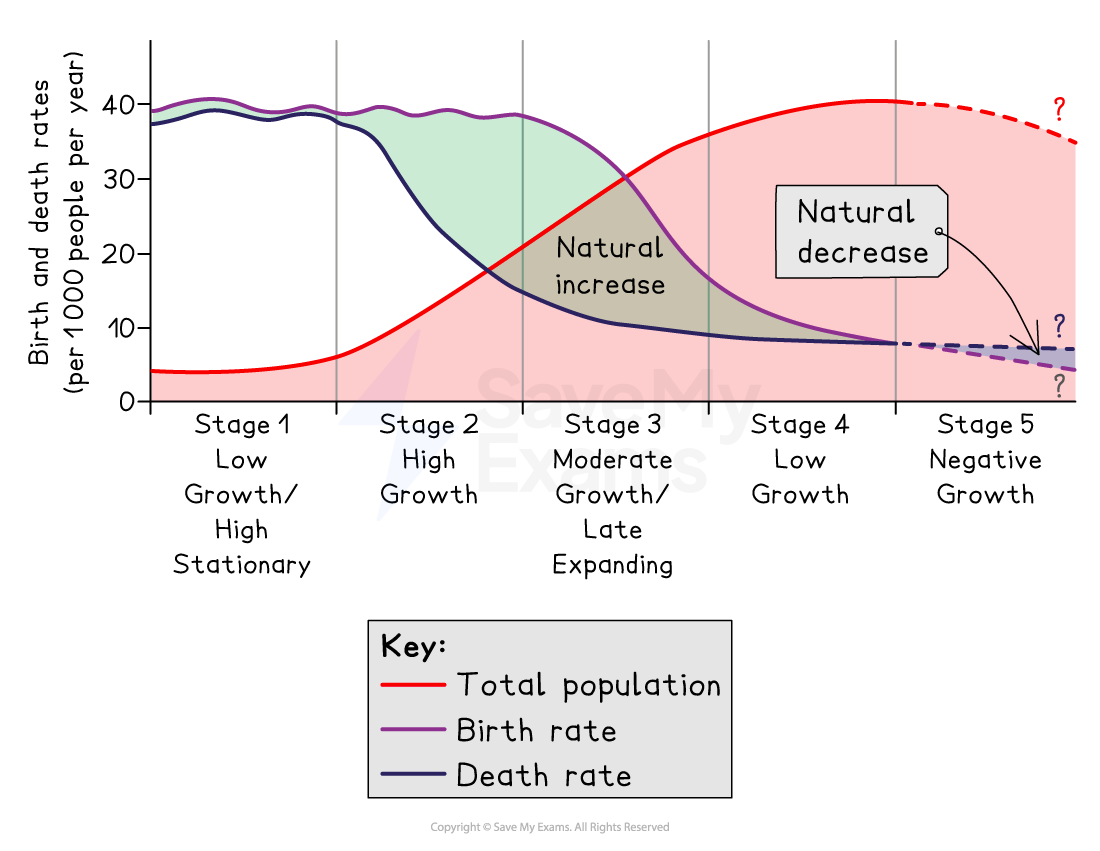
\includegraphics[width=0.9\linewidth]{transparent_5_staged.png}
    \caption{Стадии в концепции демографического перехода}
\end{figure}

Недостаток классической модели заключается в том, что она ничего не говорит о том, что происходит там, где уровень рождаемости уже стал низким, например, в странах Европы. К тому же, эта модель \textbf{не учитывает миграцию}. Для описания поведения рождаемости после завершения основной фазы перехода переходят к модели второго демографического перехода.

\begin{figure}[H]
    \centering
    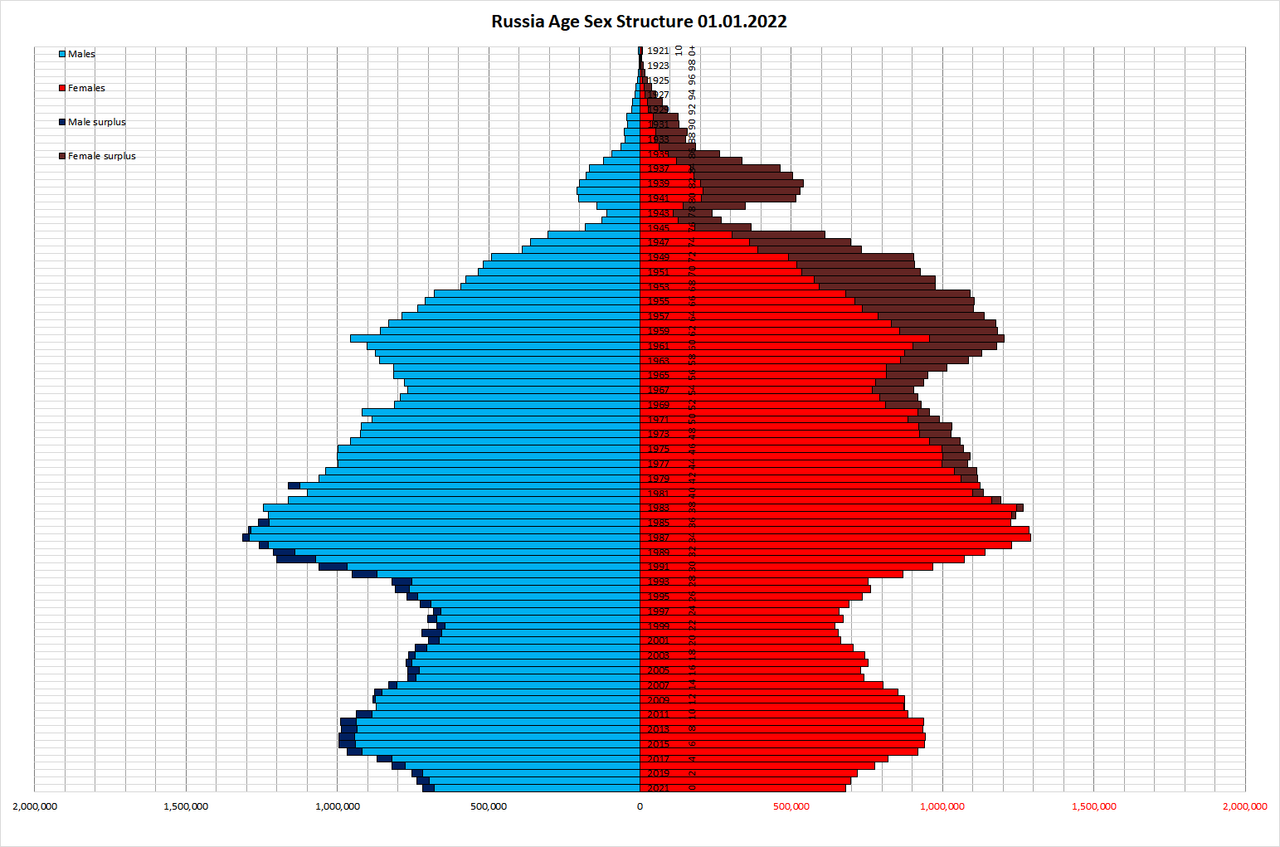
\includegraphics[width=1\linewidth]{russia.png}
    \caption{Возрастная пирамида в России}
\end{figure}

\begin{figure}[H]
    \centering
    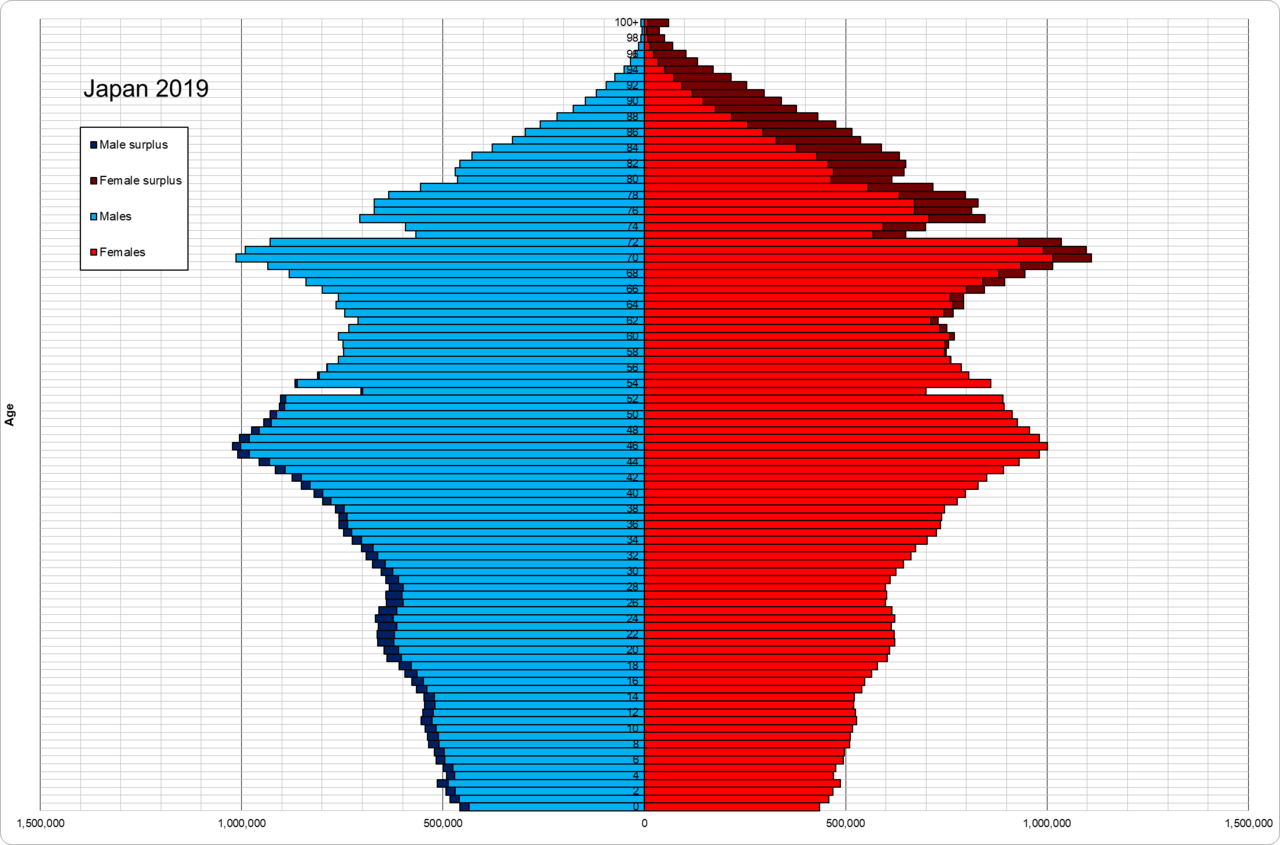
\includegraphics[width=1\linewidth]{japan.png}
    \caption{Возрастная пирамида в Японии}
\end{figure}

\textbf{Модель второго демографического перехода}, разработанная Д. ван де Каа и Р. Лестагом, относится уже не к самому началу перехода, а к обществам, где смертность и рождаемость давно стали низкими. Здесь важными становятся не только доходы или урбанизация, но и изменения семейных норм: рост возраста вступления в брак и рождения первого ребёнка, распространение незарегистрированных союзов, рост доли разводов, бездетности и откладывания родов. Поэтому на этом этапе рождаемость всё меньше зависит только от внешних экономических условий и всё сильнее --- от того, как устроены семья, нормы и жизненные планы \cite{nidi_sdt}.


\textbf{Модель затянувшегося перехода} описывает страны, где снижение смертности уже произошло, а снижение рождаемости идёт заметно медленнее из-за устойчивых социальных институтов — патриархального уклада, ранних браков, высокой ценностью детей как формы социальной страховки, слабой доступностью контрацепции, низким уровнем женского образования и слабой социальной защитой в старости. В таких случаях демографический переход не отменяется, но растягивается во времени и идёт не так быстро, как в Европе или Восточной Азии. Это особенно важно для стран Тропической Африки, где рождаемость остаётся высокой даже после заметного падения смертности \cite{owid_transition,owid_fertility}.

\section{Демографические показатели: что такое TFR?}

Модели демографического перехода описывают динамику численности насе-
ления, которая обусловлена задержкой падения рождаемости вслед за паде-
нием смертности.

Смертность в переходе снижается монотонно и прогнозируемо — на осно-
ве таблиц дожития. Рождаемость считать сложнее: из-за лага в один и тот
же календарный год живут женщины, которые уже начали снижать рождае-
мость (молодые когорты), и те, кто ещё не начал (старые когорты). Поэтому
показатель за год даёт одну картину, а за целую жизнь — другую.

В демографии различают два варианта оценки рождаемости — когортный
и периодический.

В первом случае рассматривается реальная когорта женщин одного года
рождения: сколько детей они фактически родили к завершению репродук-
тивного периода. Недостаток: измерение происходит постфактум, когда ко-
горта почти вышла из репродуктивного возраста. Такие показатели годятся
только для ретроспективного анализа.

Во втором случае берётся календарный год и суммируются возрастные
коэффициенты рождаемости, наблюдаемые в этом году. Для прогнозов ис-
пользуется периодический суммарный коэффициент рождаемости (TFR). Он
показывает, сколько детей в среднем родила бы одна женщина за всю жизнь,
если бы возрастные коэффициенты рождаемости данного года сохранялись
на всём протяжении её репродуктивного периода.

Ниже дан простой пример расчёта TFR. Пусть в 2025 году:

\begin{itemize}
    \item женщины 15 лет родили 0.005 детей на одну женщину;
    \item женщины 16 лет родили 0.010;
    \item \dots
    \item женщины 49 лет родили 0.001.
\end{itemize}

Тогда

\[
TFR_{2025} = \sum_{a=15}^{49} f_a,
\]

где $f_a$ --- коэффициент рождаемости для возраста $a$ в данном году.

Например, если в 2025 году $TFR = 1.6$, то при неизменных повозрастных коэффициентах гипотетическая женщина родит 1.6 детей за жизнь. Если в 2026 году $TFR = 1.4$, то это означает падение периодической рождаемости.

Однако TFR чувствителен к эффекту тайминга (tempo effect). Если женщины начинают рожать позже, TFR может временно снизиться даже в том случае, если итоговое число детей на женщину меняется слабее. Поэтому сам по себе TFR не всегда позволяет сразу понять, действительно ли семьи стали иметь меньше детей, или же они просто сдвинули рождение детей на более поздний возраст \cite{owid_tfr_tempo,owid_cohort_period}.

На эффекте тайминга стоит остановиться отдельно. Здесь важно не спутать пример проблемы использования показателя с описанием реальности. В жизни перенос рождения детей на более поздний возраст часто действительно связан и со снижением итоговой рождаемости когорты. Но для пояснения самого механизма удобно сначала рассмотреть предельный случай, где меняется только календарь рождений, а не их итоговое число.

\textbf{Пример А. Внезапное откладывание родов.}
Допустим, в стране женщины обычно рожали первого ребёнка в 20 лет, второго --- в 23, третьего --- в 26. Суммарно --- 3 ребёнка, то есть TFR равен 3.0.

В 2025 году происходит сдвиг к более позднему материнству. Первый ребёнок теперь рождается около 30 лет, второй --- около 33, третий --- около 36.

Что происходит с TFR в переходный момент? Женщины младших возрастов рожают меньше, чем раньше, а старшие ещё не успевают полностью компенсировать этот сдвиг. В результате количество рождений в 2025 году резко падает, и TFR снижается, скажем, до 1.5.

Что происходит с когортой? Если предположить, что эти же женщины потом всё же родят то же самое число детей, итоговая когортная рождаемость останется прежней. Значит, падение TFR в этом примере отражает не отказ от детей как таковой, а сдвиг их рождения по возрастам.

\textbf{Пример Б. Компенсация отложенных родов.}
Через некоторое время те же женщины начинают рожать позже, но более плотным потоком в старших возрастах. Тогда возрастные коэффициенты рождаемости для 30--40 лет растут, а TFR может временно подняться. Это тоже ещё не значит, что произошёл настоящий всплеск итоговой рождаемости: часть роста может быть просто компенсацией ранее отложенных рождений.

\section{Внутренние и внешние параметры моделей}

В демографических моделях параметры удобно делить на внутренние и внешние по отношению к самой модели. Внутренние параметры прямо входят в описание рождений, смертей и возрастной структуры. Внешние параметры задают условия, при которых эти внутренние величины меняются.

К внутренним параметрам обычно относят рождаемость и смертность. При этом сама рождаемость тоже может быть разложена на более простые механизмы. В модели Дж. Бонгаартса рождаемость раскладывается на несколько связанных факторов:
\[
TFR = TF \cdot C_m \cdot C_c \cdot C_a \cdot C_i,
\]
где $TF$ --- биологический максимум рождаемости, $C_m$ --- доля женщин, живущих в союзе (вообще входящих в деторождение), $C_c$ --- влияние контрацепции, $C_a$ --- влияние абортов и выкидышей, $C_i$ --- влияние послеродового перерыва между родами.

Из одного только вступления в брак не следует рост рождаемости. Смысл коэффициента $C_m$ уже: он отражает не сам факт брака, а то, насколько женщины вообще находятся в ситуации, где возможно зачатие.

Последний множитель, связанный с послеродовым периодом, особенно важен для традиционных обществ. Длительное грудное вскармливание и связанное с ним временное снижение фертильности могут заметно растягивать интервалы между рождениями.

Смертность моделируется через таблицы смертности с выделением воз-
растных интервалов. Особое значение придаётся смертности до репродук-
тивного возраста. Именно резкое увеличение числа доживающих детей по-
том создаёт тот самый демографический взрыв на ранней стадии перехода:
детей рождается по-прежнему много, но теперь гораздо больше из них дожи-
вают до взрослого возраста.

В досовременных обществах, чтобы обеспечить замещение поколений, женщине приходилось рожать много детей, поскольку смертность в детских возрастах была очень высокой. Сейчас, как только родители осознают, что дети с большой вероятностью доживут до взрослого возраста, экономическая логика многодетности постепенно рушится.

Внешние параметры подразделяются на экономические (ВВП на душу, урбанизация, стоимость жилья, занятость женщин) и институциональные (доступность образования, пенсионные системы).

Переход от многодетности к малодетности происходит тогда, когда де-
ти перестают быть «социальной страховкой» старости, а их воспитание на-
чинает требовать значительных инвестиций.

\section{Показатели воспроизводства: TFR и NRR}

Для оценки простого воспроизводства населения используют Net Reproduction Rate (NRR) - нетто-коэффициент воспроизводства. В отличие от TFR, который показывает общее число рождений на женщину при текущих возрастных коэффициентах, NRR показывает, сколько дочерей, доживающих до возраста материнства, оставляет после себя одна женщина \cite{undata_nrr}.

Почему здесь речь именно о дочерях? Потому что NRR измеряет не всё
население сразу, а замещение поколения матерей следующим поколением ма-
терей. Мальчики из расчёта не <<исчезают>>; просто для самого коэффициента
воспроизводства они не нужны. Их роль уже учтена в том, что при рожде-
нии мальчиков обычно немного больше, чем девочек.

\subsection{Строгое определение}

В непрерывной форме NRR определяется как интеграл по репродуктивному возрасту:

\begin{equation}
\text{NRR} = \int_{\alpha}^{\beta} l(x) \cdot m_f(x) \, dx
\label{eq:nrr_cont}
\end{equation}

Здесь $l(x)$ --- доля женской когорты, дожившая до возраста $x$. Например, если из 1000 новорождённых девочек до 20 лет доживают 960, то $l(20)=0.96$. Именно такие величины и берутся из таблиц смертности. Величина $m_f(x)$ --- возрастная рождаемость девочек в возрасте $x$, то есть сколько девочек в среднем приходится на одну женщину этого возраста за единицу времени.

Тогда произведение $m_f(x)\,dx$ --- это вклад очень малого возрастного интервала $[x,x+dx]$, а множитель $l(x)$ оставляет только ту долю когорты, которая до этого возраста вообще дожила.

\subsection{Дискретная форма}

Если возрастные коэффициенты заданы по годам, то
\begin{equation}
\text{NRR} = \sum_{x=a}^{b} l_x \cdot m_x^{(f)}
\label{eq:nrr_disc_new}
\end{equation}
где $a, \ b$ - нижняя и верхняя границы репродуктивного периода.

Смысл здесь простой. Берём условную когорту из 1 новорождённой девочки. До 25 лет дожила доля $l_{25}$, до 26 --- доля $l_{26}$ и так далее. Каждая из доживших женщин в возрасте $x$ рожает в среднем $m_x^{(f)}$ девочек. Значит вклад возраста $x$ в замещение равен $l_x m_x^{(f)}$. Складывая такие вклады по всем возрастам, и получаем NRR.

Пример. Пусть нас интересуют только три возраста --- 25, 26 и 27 лет. Допустим,
\[
l_{25}=0.970,\qquad l_{26}=0.969,\qquad l_{27}=0.968,
\]
а возрастные коэффициенты рождений девочек равны
\[
m_{25}^{(f)}=0.12,\qquad m_{26}^{(f)}=0.10,\qquad m_{27}^{(f)}=0.08.
\]
Тогда вклад этих трёх возрастов равен
\[
0.970\cdot 0.12 + 0.969\cdot 0.10 + 0.968\cdot 0.08 = 0.29074.
\]
То есть только за эти три года 1 новорождённая девочка, дожившая до этого возраста, оставляет после себя в среднем примерно $0.291$ дочери. Если просуммировать такие вклады по всему репродуктивному периоду, чаще всего это 15--49 лет, получится полный NRR.

Если данные заданы, например, 5-летними возрастными группами, формула та же, но к каждому коэффициенту рождаемости нужно добавить ширину интервала, то есть множитель 5.

\subsection{Связь с суммарным коэффициентом рождаемости (TFR)}

Возрастная рождаемость девочек $m_x^{(f)}$ связана с общей возрастной рождаемостью $m_x$ через долю девочек среди новорождённых:
\begin{equation}
m_x^{(f)} = m_x \cdot \pi_f.
\label{eq:sex_ratio}
\end{equation}

Здесь $\pi_f$ --- доля девочек при рождении. Обычно она близка к $0.488$, потому что при естественном соотношении полов рождается примерно 105 мальчиков на 100 девочек. Это означает, что доля девочек среди всех новорождённых равна
\[
\pi_f=\frac{100}{105+100}\approx 0.488.
\]

Подставляя \eqref{eq:sex_ratio} в \eqref{eq:nrr_disc}, получаем:
\begin{equation}
\text{NRR} = \pi_f \sum_{x} l_x \cdot m_x.
\label{eq:nrr_pi}
\end{equation}

Суммарный коэффициент рождаемости по определению равен:
\begin{equation}
\text{TFR} = \sum_{x} m_x.
\label{eq:tfr_def}
\end{equation}

Если в качестве грубой оценки принять, что вероятность дожить до основных возрастов материнства внутри репродуктивного интервала меняется не слишком сильно, можно вынести её из суммы и получить приближённую формулу
\begin{equation}
\sum_{x} l_x \cdot m_x \approx p \cdot \sum_{x} m_x = p \cdot \text{TFR},
\label{eq:approx}
\end{equation}
где $p$ --- усреднённая вероятность дожить до типичного возраста материнства.

Тогда
\begin{equation}
\text{NRR} \approx \text{TFR} \cdot \pi_f \cdot p.
\label{eq:nrr_approx}
\end{equation}

Видно, что одного TFR мало, потому что на замещение влияет ещё и смертность до возраста материнства. Поскольку $\pi_f \approx 0.488$, можно записать ещё проще:
\begin{equation}
\text{NRR} \approx \text{TFR} \cdot 0.488 \cdot p.
\label{eq:nrr_simple}
\end{equation}

\subsection{Порог простого замещения}

Рассмотрение TFR показывает, что этот показатель не является оптимальным для оценки будущего воспроизводства. Ситуация, когда $\text{TFR}>2.1$, но из-за высокой детской и подростковой смертности $\text{NRR}<1$, математически возможна.

Действительно, если использовать приближение
\[
\text{NRR} \approx \text{TFR} \cdot 0.488 \cdot p,
\]
то при $TFR=2.1$ условие $\text{NRR}<1$ даёт
\begin{equation}
2.1 \cdot 0.488 \cdot p < 1,
\label{eq:threshold1}
\end{equation}
\begin{equation}
1.0248 \cdot p < 1,
\label{eq:threshold2}
\end{equation}
\begin{equation}
p < 0.9758.
\label{eq:threshold3}
\end{equation}

То есть при такой прикидке вероятность дожить до возрастов материнства должна быть ниже примерно $97.6\%$. TFR равный 2.1 - это не строгая граница для всех стран и эпох, а именно приближение. При современной очень низкой смертности одного лишь TFR около 2.1 обычно хватает для замещения, а при заметной детской и подростковой смертности --- уже нет.

\section{Исторические и современные примеры}

Ниже приведены случаи, на которых видно, как работает грубая формула и зачем нужен переход от $TFR$ к показателям воспроизводства.

\textbf{Египет, середина 1990-х годов.}
По данным Egypt DHS 1995, суммарный коэффициент рождаемости для периода $1990$--$1995$ составлял примерно $3.65$, а смертность детей до $5$ лет --- $81$ на $1000$ рождений, то есть около $8.1\%$ \cite{egypt_rand, egypt_dhs1995_child}.

Если для грубой верхней оценки взять только выживаемость до $5$ лет,

\[
p_5 = 1-0.081 = 0.919,
\]

то получаем

\[
\text{NRR} \approx 3.65 \cdot 0.488 \cdot 0.919 \approx 1.64.
\]

Это ещё не точный $NRR$, а завышенная оценка сверху, потому что после $5$ лет смертность тоже не равна нулю. Но даже такая грубая оценка уже показывает, что до зоны незамещения Египту тогда было далеко.

\vspace{0.4cm}

\textbf{Египет, 2023 год.}
В 2023 году в Египте $TFR$ составлял $2.75$, а доля умерших до $5$ лет --- $1.8\%$ \cite{egypt_profile}.

Тогда грубая верхняя оценка даёт

\[
p_5 = 1-0.018 = 0.982,
\]

\[
\text{NRR} \approx 2.75 \cdot 0.488 \cdot 0.982 \approx 1.32.
\]

И здесь результат всё ещё выше единицы, но видно значительное снижение.

\vspace{0.4cm}

\textbf{Чад, 2023 год.}
В Чаде в 2023 году $TFR$ составлял $6.12$, а доля умерших до $5$ лет --- $10.1\%$ \cite{chad_profile}.

При грубой верхней оценке по выживанию до $5$ лет,

\[
p_5 = 1-0.101 = 0.899,
\]

\[
\text{NRR} \approx 6.12 \cdot 0.488 \cdot 0.899 \approx 2.68.
\]

даже при очень грубом счёте воспроизводство здесь многократно выше простого замещения.

\begin{figure}[H]
    \centering
    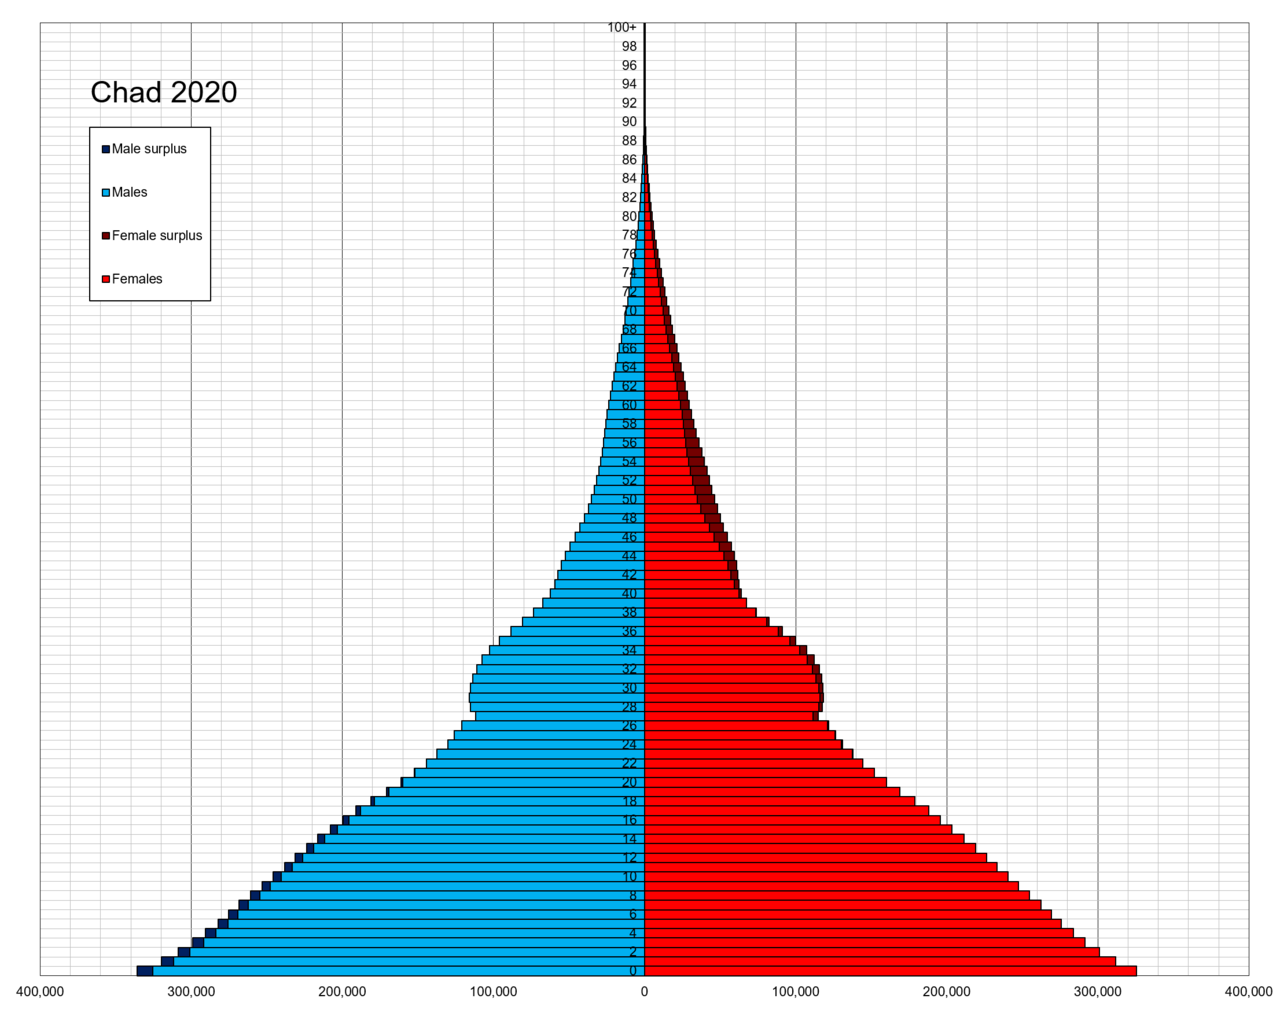
\includegraphics[width=1\linewidth]{chad_pyramide.png}
    \caption{Возрастная пирамида Чада}
    \label{Возрастная пирамида Чада}
\end{figure}

\vspace{0.4cm}

\textbf{Израиль, 2023 год.}
Израиль удобен как противоположный пример развитой страны, где рождаемость всё ещё выше уровня простого замещения. В 2023 году $TFR$ там составлял $2.83$, а доля умерших до $5$ лет --- $0.3\%$ \cite{israel_profile}.

\[
p_5 = 1-0.003 = 0.997,
\]

\[
\text{NRR} \approx 2.83 \cdot 0.488 \cdot 0.997 \approx 1.38.
\]

\vspace{0.4cm}

\textbf{Швеция, 2023 год.}
Швеция удобна как пример страны с очень низкой смертностью, но уже низкой рождаемостью. В 2023 году $TFR$ там составлял $1.43$, а доля умерших до $5$ лет --- $0.2\%$ \cite{sweden_profile}.

\[
p_5 = 1-0.002 = 0.998,
\]

\[
\text{NRR} \approx 1.43 \cdot 0.488 \cdot 0.998 \approx 0.70.
\]

Здесь уже видно обратное: даже почти полное выживание детей не компенсирует низкий $TFR$, и простого замещения нет.

\begin{thebibliography}{99}

\bibitem{owid_transition}
Roser M. \textit{Demographic transition: Why is rapid population growth a temporary phenomenon?}
Our World in Data.
\url{https://ourworldindata.org/demographic-transition}

\bibitem{owid_cohort_period}
Dattani S. \textit{Period versus cohort measures: what's the difference?}
Our World in Data.
\url{https://ourworldindata.org/period-versus-cohort-measures-whats-the-difference}

\bibitem{owid_tfr_tempo}
Dattani S. \textit{What is the total fertility rate, and how is it calculated?}
Our World in Data.
\url{https://ourworldindata.org/total-fertility-rate-births-per-woman}

\bibitem{owid_fertility}
Dattani S. \textit{Fertility Rate}.
Our World in Data.
\url{https://ourworldindata.org/fertility-rate}

\bibitem{undata_tfr}
United Nations Statistics Division.
\textit{Total fertility rate definition}.
UNdata Glossary.
\url{https://data.un.org/Glossary.aspx?q=Total+fertility+rate+%28live+births+per+woman%29}

\bibitem{undata_nrr}
United Nations Statistics Division.
\textit{Net reproduction rate definition}.
UNdata Glossary.
\url{https://data.un.org/Glossary.aspx?q=Net+reproduction+rate+%28surviving+daughters+per+woman%29}

\bibitem{nidi_sdt}
Netherlands Interdisciplinary Demographic Institute.
\textit{The Second Demographic Transition}.
NIDI.
\url{https://nidi.nl/en/nieuws_events/nidi-50-the-second-demographic-transition-1986/}

\bibitem{bongaarts_review}
Majumder N., Ram F.
\textit{Explaining the Role of Proximate Determinants on Fertility Decline among Poor and Non-Poor in Asian Countries}.
\url{https://pmc.ncbi.nlm.nih.gov/articles/PMC4331548/}

\bibitem{egypt_dhs1995_child}
Egypt Demographic and Health Survey 1995.
Chapter 9: Infant and Child Mortality.
\url{https://dhsprogram.com/pubs/pdf/FR71/09Chapter9.pdf}

\bibitem{egypt_dhs1995_full}
Egypt Demographic and Health Survey 1995.
Full report.
\url{https://www.dhsprogram.com/pubs/pdf/FR71/FR71.pdf}

\bibitem{egypt_profile}
Ritchie H. \textit{Egypt — Population and Demography Country Profile}.
Our World in Data.
\url{https://ourworldindata.org/profile/population-demography/egypt}

\bibitem{chad_profile}
Ritchie H. \textit{Chad — Population and Demography Country Profile}.
Our World in Data.
\url{https://ourworldindata.org/profile/population-demography/chad}

\bibitem{israel_profile}
Ritchie H. \textit{Israel — Population and Demography Country Profile}.
Our World in Data.
\url{https://ourworldindata.org/profile/population-demography/israel}

\bibitem{sweden_profile}
Ritchie H. \textit{Sweden — Population and Demography Country Profile}.
Our World in Data.
\url{https://ourworldindata.org/profile/population-demography/sweden}

\bibitem{owid_gender_ratio}
Ritchie H., Roser M.
\textit{Gender Ratio}.
Our World in Data.
\url{https://ourworldindata.org/gender-ratio}

\end{thebibliography}

\end{thebibliography}

\end{document}